\documentclass{article}
\title{MEC 331 Assignment 3}
\author{Odo Chinagorom. Reg  No:2018/249040 }
\usepackage{graphicx}
\begin{document}
\maketitle
\newpage

% This is for the first question
\section*{Problem 3.2}
\begin{center}\underline{Solution}\end{center}
\begin{itemize}
\item Finding the torque \newline
 Given: \[\tau =45MPa= 45 \times 10^{6}Pa\]\[r= 30mm = 0.03m\]\[R = 45mm = 0.024m\]
\[\tau = \frac{{T}{r}}{J}\]
Making $ T$ the subject of the formular
\[T = \frac{J\tau}{r} = \frac{{\frac{\pi}{2}}\times(0.045^{4} - 0.03^{4})\times 45 \times 10^{6}}{0.045} = 5.168\times 10^{3}\]
\item For solid shaft with the same cross sectional area, $A_{s} = A_{h}$
\[A_{s} = \pi(R^{2}-r^{2}) =  \pi((25\times10^{-3})^{2}-(30\times10^{-3})^{2}) = 3.5343\times10^{-3}m^{2}\]
But $A_{s} = \pi r^{2}$
\[r = \sqrt{\frac{A_{s}}{\pi}} = \sqrt{\frac{3.5343\times10^{-3}}{\pi}} = \sqrt{1.1225\times10^{-3}} = 0.0335m\]
\[\tau_{max} = \frac{{T}{r}}{J} = \frac{{T}\times{2}}{{\pi}{r^{3}}} = \frac{{5.1689\times 10^{3}}\times{2}}{{\pi}{0.033541}} = {87.2\times10^{6}Pa}\]
\end{itemize}

% This is for the second question
\section*{Problem 3.6, Page 154}
\begin{center}\underline{Solution}\end{center}
\begin{itemize}
\item 
 Given: \[\tau_{allow} = 80 \times 10^{6}Pa\]\[d_{s} = 20mm = 0.02m\]\[r = \frac{20}{2} = 10mm 10\times10^{-3}m\]
\[\tau = \frac{{T}{r}}{J}\]
Making $ T$ the subject of the formular
\[T = \frac{J\tau}{r} = \frac{{\frac{\pi}{32}}\times(0.02^{4})\times 80 \times 10^{6}}{\frac{0.02}{2}} = 125.664Nm\]
\item Assuming it becomes a hollow cylinder, $A_{s} = A_{h}$\newline
Given: \[\tau = 45 \times 10^{6}Pa\]\[r_{1} = ?\]\[r_{2} = 0.5r_{1}\]
\[ A_{s} = A_{h}\]\[\pi r^{2} = \pi({r_{2}}^{2} - {r_{1}}^{2})\]\[(10\times10^{-3})^{2} = ({r_{2}}^{2} - {r_{1}}^{2})\]
\[10\times10^{-4} = ({r_{2}}^{2} - {r_{1}}^{2}) ------------ equ(1)\]
but inner diameter equals half of the outer diameter. This implies that $r_{1} = \frac{r_{2}}{2}$
Substituting it into equ(1) above, we get
\[10\times10^{-4} = ({r_{2}}^{2} - {\frac{{r_{2}}}{2}}^{2})\]
\[10\times10^{-4} = ({r_{2}}^{2} - \frac{{r_{2}}^{2}}{4})\]
\[10\times10^{-4} = \frac{{3r_{2}}^{2}}{4}\]
Making $ {r_{2}} $ subject of the formular, we have
\[r_{2} =\sqrt{ \frac{1\times10^{-4}\times4}{3}} = \sqrt{1.333\times10^{-4}} = 0.01155m\]
\[r_{1} = 0.01154 \space \space \space , r_{2} = 0.005772\]
\[T = \frac{J\tau}{r} = \frac{{\frac{\pi}{2}}\times(0.01154^{4} - 0.005772^{4})\times 80 \times 10^{6}}{0.01154} = 181.03Nm\]
\end{itemize}


%This is for the third question.
\section*{Problem 3.10}

\begin{center}\underline{Solution}\end{center}
\begin{itemize}
\item  In Shaft AB\newline
Given: \[d = 0.03m\]\[T_{AB} = 300Nm\]\[r = \frac{d}{2} = 0.015m\]\newline
\begin{center}The formular for solving this question $\tau_{max} = \frac{T\times r}{J}$\end{center}
\[\tau_{max} = \frac{T\times r}{J} = \frac{300\times0.015}{\frac{\pi}{32}\times {0.03}^{4}} = 56.58\times10^{6}Nm\]
\item In Shaft BC \newline
Given: \[d = 0.046m\]\[T_{BC} = 400Nm + 300Nm = 700Nm\]\[r = \frac{d}{2} = 0.023m\]\newline
\[\tau = \frac{T\times r}{J} = \frac{700\times0.023}{\frac{\pi}{32}\times {0.046}^{4}} = 20.92\times10^{6}Nm\]
The highest shear stress is $ 56.58\times10^{6}Nm$ occurs in portion AB. Reduce the diameter of BC to provide the same stress
 \[T_{br} = 700Nm, \tau_{max} = \frac{T_{r}}{J} = \frac{2T}{\pi r^{3}}\]
Making $r $ subject of the formular we have that \[r^{3} = \frac{2\times T}{T\times\pi}\]
\[r = \sqrt[3]{\frac{2\times700}{56.58\times10^{6}\times\pi}} = 0.019896\]
\[d = 2r = 2\times0.019896 = 0.03979m\]

\end{itemize}


% This is for the fourth question
\section*{Problem 3.13, Page 156}

\begin{center}\underline{Solution}\end{center}
\begin{itemize}
\item Torque in Shaft BC,\newline
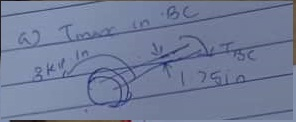
\includegraphics{IMG-20220210-WA0006}\newline
Given\[r_{2} = 0.5in, r_{1}=\frac{1.75}{2} = 0.875in, T_{BC} = 3\times10^{3}lbs.in\]
\[\tau_{max} = \frac{T\times r}{J} = \frac{3\times10^{3}\times0.875}{\frac{\pi}{2} \times (0.875^{4} - 0.5^{4})} = 3.19\times10^{3}lbs.in\]
\item Torque in Shaft CD\newline
Given\newline
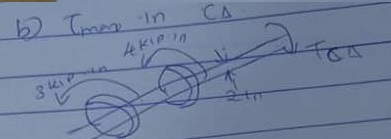
\includegraphics{IMG-20220210-WA0008}\newline
From the free body diagram, we have
\[r_{2} = 0.5in, r_{1}=\frac{2}{2} = 1in, T_{CD}=(4+3)\times10^{3} = 7\times10^{3}psi.in\]
\[\tau_{max} = \frac{T\times r}{J} = \frac{7\times10^{3}\times1}{\frac{\pi}{2} \times (1^{4} - 0.5^{4})} = 4.75\times10^{3}psi.in\]
\item In Shaft DE\newline
Given \newline
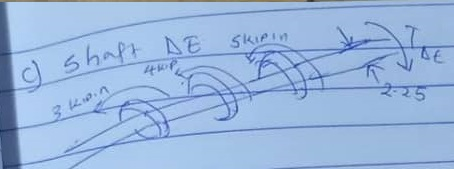
\includegraphics{IMG-20220210-WA0009}\newline
\[r_{2} = 0.5in, r_{1}=\frac{2.25}{2} = 1.125in, T_{DE}=(4+3+5)\times10^{3} = 12\times10^{3}psi.in\]
\[\tau_{max} = \frac{T\times r}{J} = \frac{12\times10^{3}\times1.125}{\frac{\pi}{2} \times (1.125^{4} - 0.5^{4})} = 5583.36psi.in\]
\end{itemize}


%This is for the fifth Problem
\section*{Problem 3.18}


\begin{center}\underline{Solution}\end{center}
Since the factor of safety is the same for each of them, 
\begin{center}$T_{s} = T_{b} = $ Largest Torque\end{center}
Given: \[T_{s} = 25\times10^{6}Nm, r= 0.015m\]
\[T_{s} = \frac{\tau_{allow}\times J}{r} = \frac{25\times10^{6}\times\frac{\pi}{2}\times{0.015}^{4}}{0.03} = 132.53Nm\]
Finding the inner diameter of the brass, we have
\[T_{b} = \frac{\tau_{b}\times\frac{\pi}{2}\times({r_{1}}^{4}-{r_{2}}^{4})}{r_{1}} \]
Given:\[T_{b} = 25\times10^{6}Nm, r= 0.0125m\]
\[r = \sqrt[4]{{r_{1}}^{4} - \frac{2\times T_{b}\times r_{1}}{\pi\times\tau}}= \sqrt[4]{{0.0125}^{4} - \frac{2\times132.5\times 0.0125}{\pi\times50\times10^{-3}}} = 0.00759\]
\[d = 2r = 0.01518m\]
The largest Torque is $T_{allow} = 132.5Nm$

%This is for the sixth Problem
\section*{Problem 3.32}


\begin{center}\underline{Solution}\end{center}
Given \[\phi =4^{o} = 0.06981rad, G = 27\times10^{9}Pa, l = 1.25m, r_{1} = 0.018m, r_{2} = 0.012m\]
\[T = \frac{\phi J G}{L} = \frac{0.06981\times\frac{\pi}{2}\times(0.018^{4}-0.012^{4})\times27\times10^{9}}{1.25} = 199.53Nm\]
Matching areas. Hence, \[A_{c}=A_{h}\]
\[\pi r^{2} = \pi({r_{2}}^{2} - {r_{1}}^{2})\]
\[ r^{2} = ({r_{2}}^{2} - {r_{1}}^{2})\]
Making r the subject of the formular, we have
\[ r^{2} = {({1.8\times10^{-3}}^{2} - {2\times10^{-3}}^{2})}\]
\[r = \sqrt{\frac{5.654\times10^{-4}}{\pi}}=0.0134m\]
The angle of twist is 
\[\phi = \frac{TL}{JG} = \frac{199.53\times1.25}{\frac{\pi}{2}\times0.0134^{4}\times27\times10^{9}} = 0.1825rad\]



% This is for the seventh Problem
\section*{Problem 3.36}


\begin{center}\underline{Solution}\end{center}
For Shaft BC\newline
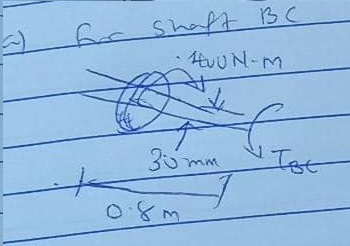
\includegraphics{IMG-20220210-WA0014}\newline
Given:  \[ G = 27\times10^{9}Pa, l = 1.25m, r_{1} = 0.015m, T_{BC} = 400Nm, L = 0.8m\]
 
\[\phi_{BC} = \frac{T_{BC}L}{JG} = \frac{400\times0.8}{\frac{\pi}{2}\times0.015^{4}\times27\times10^{9}} = 0.1490\]
\newline at D and B
\[\phi_{BD} = \phi_{BC} + \phi_{CD}\]
Given: \newline
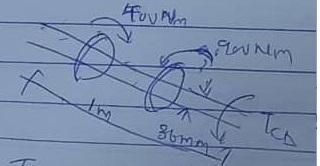
\includegraphics{IMG-20220210-WA0016}\newline
 \[ G = 27\times10^{9}Pa, l = 1.25m, r = 0.018m, T_{CD} = 400Nm - 900Nm = -500Nm , L_{CD} = 1m\]
\[\phi_{BC} = \frac{T_{CD}L_{CD}}{JG} = \frac{-500\times1}{\frac{\pi}{2}\times0.018^{4}\times27\times10^{9}} = -0.1123\]

\[\phi_{BD} = 0.182 + (-0.1123) = 0.0367rad\]


%This is for the eight question
\section*{Problem 3.40}
\begin{center}\underline{Solution}\end{center}
\[d_{s} = 1.75in, d_{b} = 3in, \phi = 0.375^{o},L_{sleeve} = 8in\]
\[G_{s} = 11.2\times10^{6}Psi, G_{b} = 5.6\times10^{6}Psi\]
\[ {{\tau_{all}}_{s}}=12ksi = 12\times10^{3}Psi,  {{\tau_{all}}_{b}}=12ksi = 7\times10^{3}Psi\]
Torque based on shear stress of the spindle
\[\tau_{all} = \frac{Tr_{s}}{J_{s}} \Rightarrow T = \frac{\tau J_{s}}{r_{s}}\]
\[T = \frac{12\times10^{3}\times\frac{\pi}{2}\times{0.875}^{4}}{0.875} = 12628.11Ibs.in\]
Torque based on sleeve 
\[d_{B1} = 3in\]
\[d_{B2} = 3-2t = 3-2(0.25) = 2.5\]
\[r_{B1} = \frac{d_{B1}}{2} = 1.5in\]
\[r_{B2} = \frac{d_{B2}}{2} =1.25in\]
\[J = \frac{\pi}{2}(1.5^{4} - 1.25^{4}) = 4.1172\]
\[T = \frac{7\times10^{3}\times4.1172}{1.5} = 19213.6lbs.in\]
Torque based on angle of rotation of sleeve
\[\phi = 0.375^{o} = \frac{0.325}{180} = 6.545\times10^{-3}\]
\[\phi = \frac{TL}{GJ} \Rightarrow T= \frac{GJ\phi}{L} = \frac{5.6\times10^{6}\times4.1172\times6.545\times10^{-3}}{8} = 18862.93lbs.in\]
The largest torque that can be applied not exceed the stresses and the angle of halt = $12628.11ibs.in$
\[L = 13, T = 12628.11\]
\[\phi = \frac{TL}{GJ} = \frac{12628.11\times13}{11.2\times10^{6}\times0.920} = 0.0147rads\]


%This is for the nineth questiion
\section*{Problem 3.44}

\begin{center}\underline{Solution}\end{center}
Givens: \[t = 5ib.in, l=2.4in, c=\frac{1}{2}d = \frac{1}{32}in, G = 11.2\times10^{6}psi, n = 2, J = \frac{\pi}{2}c^{4} =  \frac{\pi}{2}{(\frac{1}{32})}^{4} = 1.49803\times10^{-6}in^{4}\]
\begin{center}The formular is $\phi = \frac{Tl}{GJ}(1 + \frac{1}{n^{2}}+  \frac{1}{n^{4}})$\end{center}
\[\phi = \frac{5\times2.4}{11.2\times10^{6}\times1.49803\times10^{-6}}(1 + \frac{1}{4^{2}}+  \frac{1}{16^{4}}) = 938.73\times10^{-3}rad\]
\begin{center} The angle through which end A rotates in degress is $53.8^{o}$\end{center}



%This is for the tenth question
\section*{Problem 3.48}


\begin{center}\underline{Solution}\end{center}
\[T = rP = (0.3)(600) = 180N.m\]
Shaft of diameter based on displacement limit, we have based on the angle of displacement,
\[\phi = \frac{\sigma}{r} = \frac{15}{300} = 0.005 rad\]
\[\phi = \frac{TL}{GJ} = \frac{2TL}{\pi Gr^{4}}\]
\[r^{4} = \frac{2TL}{\pi\phi G} = \frac{2\times180\times0.5}{\pi\times11\times10^{9}\times0.05} = 14.882\times10^{-9}m^{4}\]
\[r = 11.045\times10^{-3}m = 11.045m\]
\[d  =2r = 22.1mm\]
Shaft diameter based on stress 
\[\tau = 80\times10^{6}Pa\]
\[\tau =\frac{Tr}{J}=\frac{2T}{\pi r^{3}}\]
\[r = \sqrt[3]{\frac{2T}{\pi\tau} }= \frac{(2)(180)}{\pi(80\times10^{6})} = \sqrt[3]{1.43239\times10^{-6}m^{3}} = 11.273\times10^{-3}m = 11.273mm\]
\[d = 2r = 22.5mm\]
Use the larger value to meet both limits
\end{document}